We will now give a basic review of lung physiology. A more complete introduction can be found in \citet{west2008respiratory,cotes2009lung}.
 
\subsection{Mechanics of breathing} 
During inspiration, the volume of the thoracic cavity increases and air is drawn into the lung by creating a sub-atmospheric pressure distribution. The increase in volume is brought about mainly by contraction of the diaphragm, which causes it to descend, and partly by the action of the intercostal muscles, which raise the ribs. 
The lung is elastic and subsequently returns passively to its preinspiratory volume during resting breathing. During expiration the intra-alveolar pressure becomes slightly higher than atmospheric pressure and gas flows out of the
lungs \citep{west2008respiratory}. 
%The pressure required to move gas through the airways in a healthy lung is very small. During normal inspiration, an air flow rate of $1$ liter per second requires a pressure drop along the airways of less than $200$ Pa. Compare this to a smoker’s pipe, which needs a pressure of about $50,000$ Pa for the same flow rate \citep{west2008respiratory}.

\subsection{Airway tree} 
The airway tree is divided into a conducting zone and a respiratory zone. The trachea divides into right and left main bronchi, which in turn divide into lobar and then segmental bronchi. This process continues down to the terminal bronchioles, which are the smallest airways without alveoli. All of these bronchi make up the conducting airways. %An image of the conducting airway tree is shown in Figure \ref{fig:rubber_tree}. 
The terminal bronchioles, which appear at around generation 15-16, then continue to divide into respiratory bronchioles, which have occasional alveoli budding from their walls. Finally, we get to the alveolar ducts, which are completely lined with alveoli, see Figure \ref{fig:honey}. This alveolated region of the lung where the gas exchange occurs is known as the respiratory zone \citep{west2008respiratory}. Table \ref{table:tree} documents the different flow characteristics found in the airway tree during slow and rapid breathing.
%
%
\begin{figure}[H]
  \begin{center}           
  \subfloat[]{\label{fig:honey}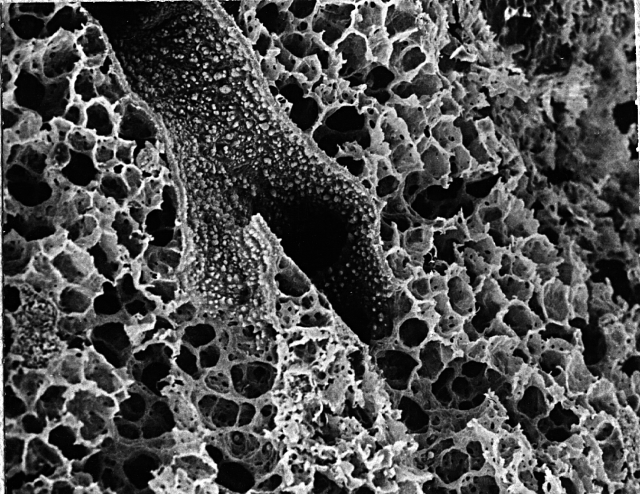
\includegraphics[width=0.35\textwidth,height=2.0in]{figures/images/TB_to_aveolarduct_BerkeleyLungLabtour.png}}
   \subfloat[]{\label{fig:pores}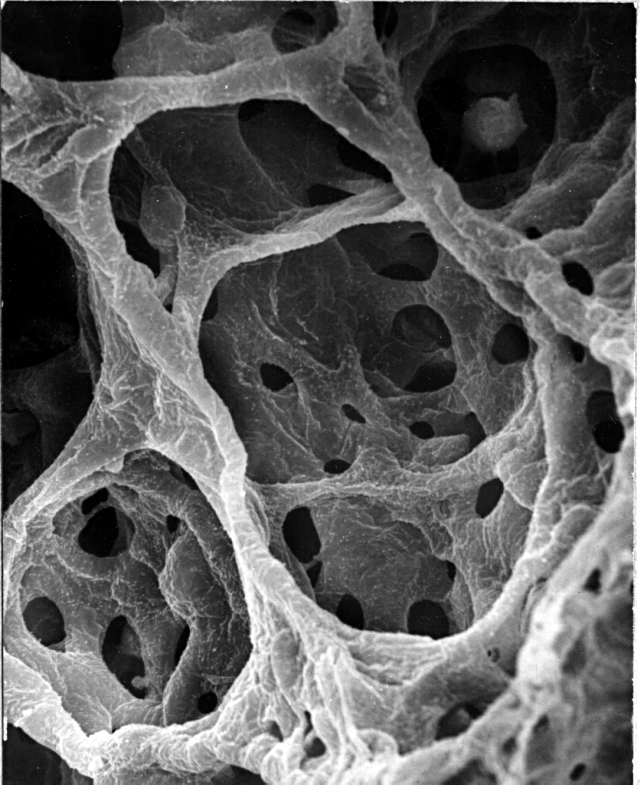
\includegraphics[width=0.35\textwidth,height=2.0in]{figures/images/aveolarPores_BerkeleyLungLabLungtour.png}}     \\
   \subfloat[]{\label{fig:sponge}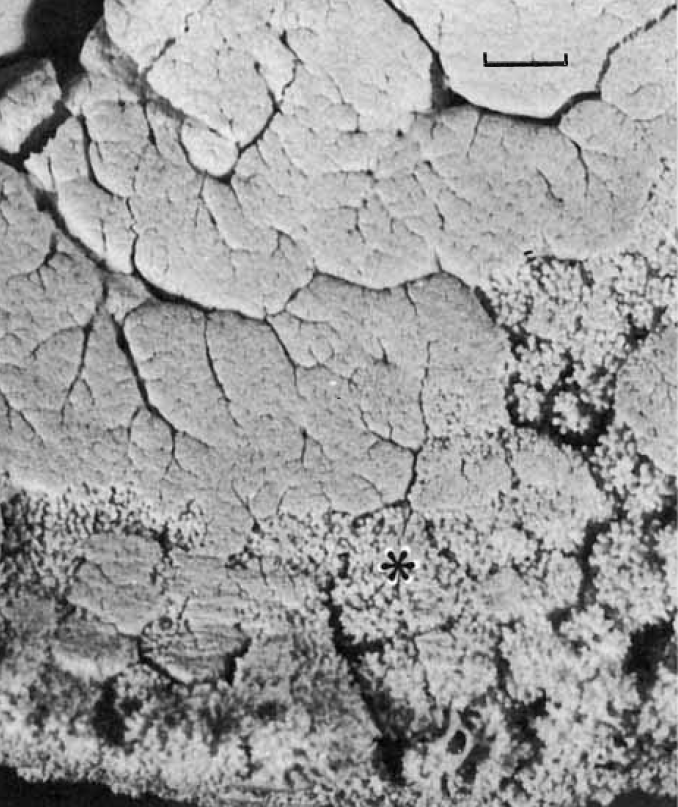
\includegraphics[width=0.35\textwidth,height=2.0in]{figures/images/upperlobe_haefeli1988.png}}  
\subfloat[]{\label{fig:acini}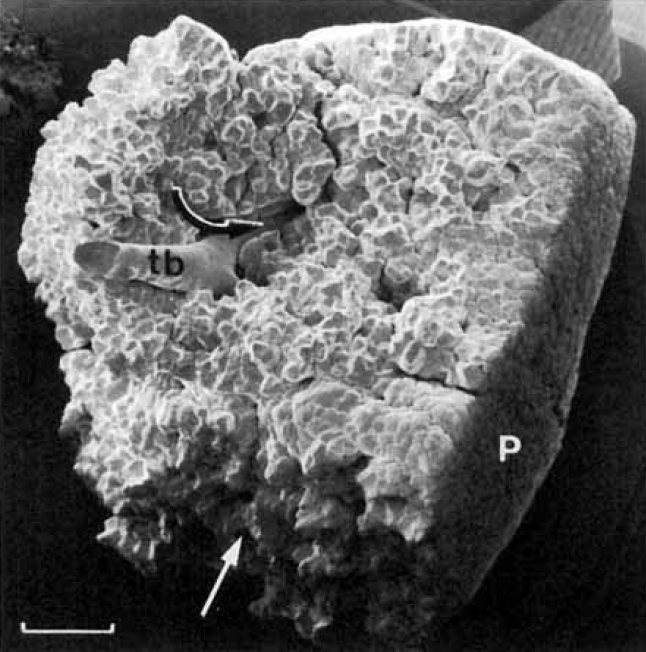
\includegraphics[width=0.35\textwidth,height=2.0in]{figures/images/acinus_HAEFELI-BLEUER1988.png}}
\caption{(a) Transition from terminal bronchiole to alveolar duct, from conducting airway to oxygen transfer area, diameter of terminal bronchiole is $0.5 \;\mbox{mm}$. (b) A few alveoli in an alveolar duct. The dark round openings are pores between alveoli. The alveolar wall is quite thin and contains a network of capillaries. The average diameter of one alveoli is $0.2\;\mbox{mm}$.  (c) Portions of silicone rubber casts of upper lobes
of human lungs; asterisk marks incompletely filled regions. The outline of individual unfilled acinar units can also be seen. Scale marker, $5\;\mbox{mm}$. (d) Scanning electron micrograph of complete acinus with transitional bronchiole
(tb) and surface abutting on pleura (P). Note the irregular surface where alveolar sacs of adjacent acini interdigitate (straight arrow). Scale marker, 1 mm. Images are reproduced from \citet{lunglabshort}.
 }
  \end{center}
   \label{fig:acinar_units}
\end{figure}
%
\begin{table}[h]
\begin{center}
\scalebox{0.76}{
\begin{tabular}{|l|c|c|c|c|c|c|}
\hline
Generation & Diameter & Length  & Flow rate 10L/min & Re & Flow rate 100L/min & Re \\
           & cm            & cm         &Velocity (m/s) &  & Velocity (m/s) & \\

\hline 
Trachea & 1.80 & 12.0 & 65.8 & 775 & 658 & 7750  \\
1 & 1.22 & 4.76 & 71.6 & 573 & 716 & 5730\\
5 & 0.35 & 1.07 & 53.6 & 123 & 536 & 1230\\
10 & 0.13 & 0.46 & 12.55 & 10.6 & 125 & 106\\
15 & 0.066 & 0.20 & 1.48 & 0.63 & 14.8 & 6.30\\
20 & 0.045 & 0.083 & 0.10 & 0.031 & 1.00 & 0.31\\

\hline
\end{tabular}
}
\end{center}
\caption{Shows dimensions, velocity and the corresponding Reynolds number for different sections of the airway tree during slow and rapid breathing. 
%Terminal bronchioles appear at around generation 15-16 which are then followed by respiratory bronchioles, the first generation to have alveoli. 
These values have been taken from \citet{pedley1970prediction}. }
\label{table:tree}
\end{table}
%
\begin{figure}[H]
  \centering
{\label{fig:mouse}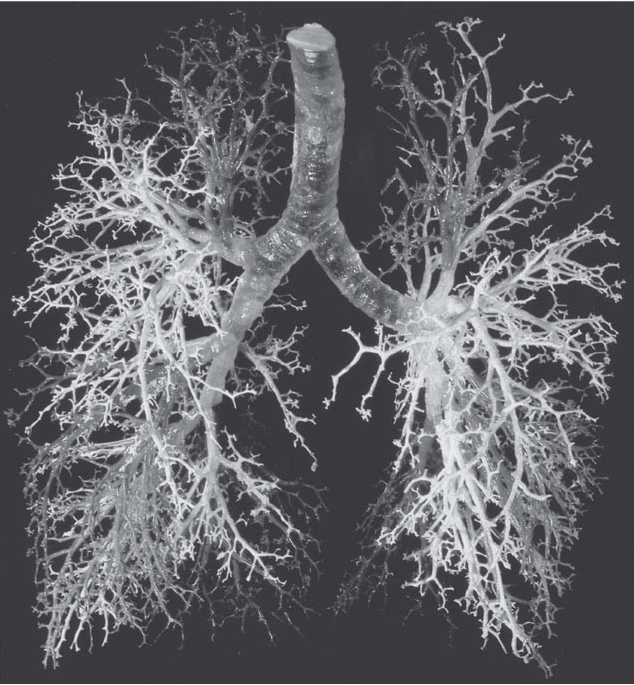
\includegraphics[width=0.5\textwidth]{figures/images/lung_west.pdf}}                
  \label{fig:acinar_units}
\caption{A rubber cast of the conducting airways of a human lung. The image is reproduced from \cite{west2008respiratory}.}
\label{fig:rubber_tree}
\end{figure}

\subsection{Lung parenchyma} 
 Lung parenchyma refers to the portion of the lung made up of the small air chambers (alveoli) participating in gas exchange. The alveoli are made up of collagen, elastin fibers and membranous structures containing the capillary network, see Figure \ref{fig:pores}. Alveoli are arranged in sponge like structures and fill the entire volume of the lungs surrounding the conducting passages. Figure \ref{fig:sponge} shows a rubber cast of lung parenchyma, the dark lines outline the branching structure of the airways.
%The interior design of lung parenchyma is determined by the branching of the conducting airways. 
The right and left lung are partitioned into three and two lobes, respectively. Lung segments of conic shape are then the first subdivision of these lobes. These structures are bounded by connective tissue such that surgical separation is often possible. In the right lung, there are usually ten segments whereas only nine can be found in the left lung. Within the segments, the bronchi branch about six to twelve times. The terminal bronchioles which appear after roughly $15-16$ branching generations then finally feed into approximately $30,000$ so-called acini, see Figure \ref{fig:acini}. These acini represent the largest lung units of which all airways are alveolated and thus participate in gas exchange \citep{WeichertThesis}.



\subsection{The diseased lung}
There exist numerous ways in which the mechanical function of the lung can be altered. In this section we will briefly describe pulmonary fibrosis, emphysema, and airway constriction.


Pulmonary fibrosis is a so-called restrictive diseases. Here, abnormal deposition and organization of connective proteins, particularly collagen, leaves lung tissue scarred and stiff with with compliance values decreasing to $20\%$ of normal values \citep{bates2009lung,cotes2009lung}


Emphysema is characterized by an abnormal, permanent enlargement of air spaces distal to the terminal bronchioles and the destruction of their walls associated with loss of the elastic connective tissue. Large areas of lung tissue completely break down leaving big holes, see Figure \ref{fig:emphysemic}. This results in a reduced area for gas exchange and a reduction in the elastic recoil of the lungs. 

Airway constriction, which occurs in asthma and COPD, changes airway resistance patterns. The level of airway resistance is sensitive to disease in the lungs. Narrowing of the airways can be caused through various mechanisms such as the airway inflammation or bronchoconstriction observed in asthma, mucous hyper-secretion and inflamed bronchi observed in chronic bronchitis, or the flaccid airways observed in emphysema \citep{HedgesThesis}. This decrease in airway radius can significantly increase the resistance to flow.

%A reduction in the compliance results in a stiffer lung with a larger change in pressure required to produce a normal volume change. This condition is indicative of fibrosis where the compliance of the lung can be reduced to approximately 0.05 L/cmH2O (Hyatt et al. 2003). Sufferers of this disease have trouble inflating the lung. 
%Conversely, a lung with increased compliance results in large changes in volume for a normal change in pressure. This is observed in patients with emphysema where the compliance can be increased to more than 0.5 L/cmH2O (Hyatt et al. 2003). These patients have no difficulty inflating their lungs, however exhalation becomes difficult, due to airtrapping.






\begin{figure}[H]
  \centering
{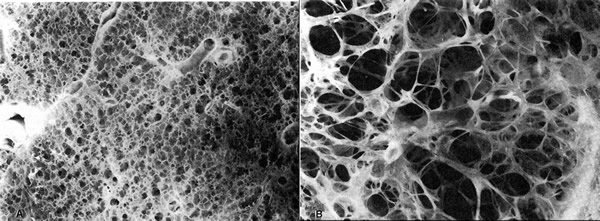
\includegraphics[width=0.9\textwidth,height=2.2in]{figures/images/emphysema.jpg}}                
 % \label{fig:emphysemic}
\caption{ Left, a cross section of healthy parenchyma. Right, a cross section of diseased (emphysemic) lung parenchyma, with big holes appearing. Images are reproduced from G. Snell, ctsnet.org.
 }
 \label{fig:emphysemic}
\end{figure}












%
%
\begin{comment}
\subsection{Collateral ventilation.} 
Need to get a copy of the following paper:
``Collateral ventilation.
Menkes H, Traystman R, Terry P.
Abstract: Ventilation may bypass obstructed airways through collateral channels, including interalveolar pores of Kohn, bronchiole-alveolar communications of Lambert, and interbronchiolar pathways of Martin. Resistance through these channels, like resistance through small airways, increases with decreasing lung volume and with hypocapnia. But whereas the distention of collateral channels and small airways by a variety of factors is similar, the efficiency of ventilation through collateral channels is less than the efficiency through airways. Gas inspired through collateral channels is contaminated with alveolar gas from surrounding lung so that the dead space for collateral ventilation is increased. When one part of the lung ventilates out of phase with the surrounding lung, pulmonary interdependence promotes more homogeneous ventilation. In the presence of airways obstruction, interdependence may be a primary factor governing the rate of collateral ventilation. In man, collateral ventilation is unimportant in normal lungs. However, with disease, it may be critical in producing or compensating for abnormalities. For example, the long time constant for collateral ventilation in the middle lobe may be responsible for atelectasis, which results in the middle lobe syndrome. On the other hand, the short time constant for collateral ventilation in emphysema may be essential for the distribution of ventilation beyond obstructed airways.''

Also need to get:
``Collateral Ventilation and Gas Exchange during Airway Occlusion in the Normal Human Lung
Nicholas W. Morrell, C. Michael Roberts, Tony Biggs, and W. Anthony Seed''
\end{comment}
\begin{comment}

\begin{table}[H]
\begin{center}
\scalebox{0.7}{
\begin{tabular}{ l c c c c c}
\hline Parameter &  Description & Value& Reference  \\
\hline
$\rho^{s}$ & Density of alveolar tissue & ${1065\;\mbox{kg}}\,\mbox{m}^{-3}$ & \cite{hogg1969regional} \\
$\rho^{s}$ & Density of the alveolar wall & ${1000\;\mbox{kg}}\,\mbox{m}^{-3}$ & \cite{lande2006analysis}\\
$\rho^{f}$ & Density of of air at 27C$^\circ$ & ${1.18 \;\mbox{kg}}\,\mbox{m}^{-3}$ & Wiki \\
$\phi_{0}$ & Estimated reference porosity in the lung & $0.93$ & \cite{WeichertThesis} \\
$\mu^{f}$ & Viscosity for air at 27C$^\circ$ & $1.86 \times 10^{-5} \; \mbox{kg}\,\mbox{m}^{-1}\,\mbox{s}^{-1}$ & Wiki \\
$\bb{\kappa} $ &Permeability of the porous media (rough approximation) & $10^{-10}-10^{-12} \; \mbox{m}^{2}$ & \cite{owen2001mechanics},\cite{lande2006analysis}\\
$p $ &Mean airway pressure
 for high-frequency oscillation & $2000 \; \mbox{kg}\,\mbox{m}^{-1}\,\mbox{s}^{-2}$ & \cite{owen2001mechanics} \\
 $\hat{v} $ & Poisson ratio of porous lung at airway pressure $2000\,\mbox{Pas}$& $0.3$ & \cite{owen2001mechanics} \\
 
  $E $ & Young's modulus of lung tissue at airway pressure $2000\,\mbox{Pas}$& $8000$ $\mbox{kg}\,\mbox{m}^{-1}\,\mbox{s}^{-2}$  & \cite{owen2001mechanics} \\
  
  $\bb{u}^{s} $ & Tissue displacement near the diaphragm assuming sinusoidal motion & $0.05$ $\mbox{m}$  & \cite{gorman2002diaphragm} \\

  $\bb{a}^{s} $ & Tissue acceleration near the diaphragm assuming sinusoidal motion & $0.02$ $\mbox{m}\,\mbox{s}^{-2}$  & calculated \\

\hline
\end{tabular}
}
\end{center}
\caption{A collection of various parameters and typical values associated with lung parenchyma.} \label{tab:summary_equations}
\label{tab:parameters}
\end{table}
\end{comment}
%